\documentclass[conference]{IEEEtran}
\IEEEoverridecommandlockouts
% The preceding line is only needed to identify funding in the first footnote. If that is unneeded, please comment it out.
\usepackage{dblfloatfix} % To enable figures at the bottom of page
\usepackage{cite}
\usepackage{algorithm}
\usepackage{algpseudocode}
\usepackage{amsmath}
\usepackage{amssymb}
\usepackage{subcaption}
\usepackage{graphicx}
\usepackage{textcomp}
\usepackage{multirow}
\usepackage{multicol}
\usepackage{xcolor}
\usepackage{amsmath}
\usepackage{comment}

\usepackage{tikz}
\usetikzlibrary{shapes.geometric, arrows.meta, positioning, calc, fit, backgrounds, shadows}

\def\BibTeX{{\rm B\kern-.05em{\sc i\kern-.025em b}\kern-.08em
    T\kern-.1667em\lower.7ex\hbox{E}\kern-.125emX}}

\def\BibTeX{{\rm B\kern-.05em{\sc i\kern-.025em b}\kern-.08em
    T\kern-.1667em\lower.7ex\hbox{E}\kern-.125emX}}
    

\makeatletter
\newcommand{\linebreakand}{%
  \end{@IEEEauthorhalign}
  \hfill\mbox{}\par
  \mbox{}\hfill\begin{@IEEEauthorhalign}
}
\makeatother


\begin{document}

\title{Deep Reinforcement Traffic Congestion and Anomaly Detection\\
% \thanks{979-8-3315-1504-1/25/\$31.00 ©2025 IEEE}
}
% author names and affiliations
% use a multiple column layout for up to three different
% affiliations
\author{\IEEEauthorblockN{Khushi}
\IEEEauthorblockA{SCSET, Bennett University\\ Greater Noida, UP, India\\
khushi@gmail.com}
\and
\IEEEauthorblockN{Jatin}
\IEEEauthorblockA{SCSET, Bennett University\\ Greater Noida, UP, India\\
jatin@gmail.com}
% \linebreakand
\and
\IEEEauthorblockN{Jaismeen}
\IEEEauthorblockA{SCSET, Bennett University\\ Greater Noida, UP, India\\
jaismeen@gmail.com}
\and
\IEEEauthorblockN{Susmita Das}
\IEEEauthorblockA{SCSET, Bennett University\\ Greater Noida, UP, India\\
susmitad900@gmail.com}}

% make the title area
\maketitle

% As a general rule, do not put math, special symbols or citations
% in the abstract
\begin{abstract}
Urban traffic congestion remains a critical bottleneck in smart city infrastructure, inducing severe economic and environmental penalties. Traditional actuated and fixed-time controllers fail to adapt to macro-level stochastic perturbations inherent in real-world traffic networks. In this paper, we present an end-to-end cyber-physical framework leveraging a Graph-Aware Dueling Double Deep Q-Network (D3QN) for multi-agent signal phase optimization, seamlessly integrated with the advanced ARGUS video anomaly detection engine. Addressing the limitations of legacy vision systems, proposed framework provides robust, zero-label self-supervised video anomaly detection explicitly designed for complex vehicular environments using the UA-DETRAC traffic surveillance dataset. The framework employs VideoMAE for high-fidelity spatio-temporal feature extraction, producing highly discriminative 768-dimensional embeddings. These embeddings are mathematically mapped through Multi-Level Density Estimation (MULDE) using denoising score matching, followed by Gaussian Mixture Model (GMM) calibration for stable, threshold-agnostic anomaly scoring. The calibrated continuous anomaly scores are natively concatenated into the D3QN state vector, empowering the reinforcement learning agent to jointly optimize for traffic congestion reduction and anomalous event mitigation. The system preserves operator-facing counterfactual transparency via Shapley Additive Explanations (SHAP) and guarantees operational safety through a deterministic cybersecurity validation gate. Ultimately, this framework demonstrates that multimodal deep reinforcement learning can be effectively synthesized with density-based computer vision for resilient, real-world deployment.
\end{abstract}

\begin{IEEEkeywords}
Adaptive traffic signal control, reinforcement learning, Dueling Double DQN, Video anomaly detection, Vision Transformer, Multi-Level Density Estimation.
\end{IEEEkeywords}

\section{Introduction}
Urban traffic congestion represents one of the most economically and environmentally damaging inefficiencies in modern metropolitan infrastructure. Global estimates place the annual cost of gridlock at over \$1.7 trillion, driven by lost productivity, wasted fuel, increased logistics overhead, and elevated vehicular carbon emissions. The near-ubiquitous reliance on legacy, deterministic traffic signal controllers operating on pre-programmed cyclic phases constitutes a primary architectural flaw. These static systems are structurally incapable of adapting to the stochastic dynamics inherent in real-world traffic environments: asymmetric rush-hour load distributions, sudden roadway incidents, and multi-modal emergency vehicle routing. Critically, conventional systems lack native mechanisms for macro-level predictive horizon planning, reacting merely to instantaneous local sensor readings. 

The field of artificial intelligence-driven traffic signal control has evolved through several distinct phases. Early rule-based adaptive systems introduced actuated control, modifying cycle lengths based on upstream occupancy sensors. However, modern research has extensively validated Reinforcement Learning (RL) as a highly effective paradigm for adaptive traffic signal control. While Multi-Agent Reinforcement Learning (MARL) paradigms employing Graph-Aware Dueling Double Deep Q-Networks (D3QN) have demonstrated significant efficacy in spatial coordination and delay reduction, they traditionally rely exclusively on numerical traffic state matrices (e.g., queue lengths, waiting times). This unimodal state representation critically fails when unquantified, anomalous physical events—such as vehicular collisions, illegal lane occupations, or erratic pedestrian crossings—disrupt the standard flow parameters.

To bridge such an extreme translational gap between isolated numerical traffic control and real-world visual chaos, this paper proposes a comprehensive, multi-modal cyber-physical system that integrates the D3QN signal optimization agent with the proposed architecture anomaly detection framework The proposed architecture synthesizes high-fidelity anomaly scores for unconstrained video streams using the UA-DETRAC surveillance dataset. The self-supervised spatio-temporal Vision Transformer (VideoMAE) pipeline is used to calibrate the Gaussian Mixture Model (GMM) in Multi-Level Density Estimator (MULDE). The calibrated continuous anomaly scores dynamically extend the D3QN observation space, thus allowing the controller to enact evasive or mitigative phase shifts in the case of catastrophic events, while optimizing standard throughput. Moreover, the framework also includes live Shapley Additive Explanations (SHAP) for continuous algorithmic auditability bounded by a deterministic cybersecurity gate to intercept adversarial or catastrophic RL actions.

The primary contributions of this paper are summarized as follows:
\begin{itemize}
    \item A fully integrated cyber-physical framework merging MARL-based D3QN traffic optimization with the proposed multimodal framework zero-label video anomaly detection engine.
    \item We propose a mathematically rigorous visual processing pipeline for spatio-temporal feature extraction based on VideoMAE and denoising score-based density estimation with MULDE. We evaluate our method on the challenging UA-DETRAC dataset.
    \item A multimodal state fusion mechanism that concatenates GMM-calibrated visual anomaly scores into the numerical D3QN state vector, enabling real-time context-aware phase switching.
    \item Ensuring hard safety guarantees and explainability via a deterministic cybersecurity validation gate and SHAP-based counterfactual transparency.
\end{itemize}

\section{Proposed Framework}

During empirical evaluation, VideoMAE embeddings were extracted offline and stored as cached 768-dimensional feature representations. Reinforcement learning optimization was performed on the recovered feature space, while the online perception pipeline was preserved as a deployment architecture.

\label{sec:proposed_framework}

The proposed system tightly couples semantic compression computer vision with deep reinforcement learning to tackle the intrinsic volatility of urban transportation networks. The framework performs a continuous forward pass from raw pixel ingestion to optimal phase actuation, rather than treating visual anomaly detection and traffic signal control as mathematically distinct areas.

\subsection{Layered Architecture and Total Pipeline}
The system architecture is a sequential multimodal pipeline where the goal is to convert high-dimensional video streams to low-dimensional actionable anomaly scores that then condition the D3QN policy. The logical pipeline is composed of the following hierarchical stages:

\paragraph{Traffic Surveillance Videos}
The framework is intended to take unconstrained, real-world traffic surveillance video data collected directly from UA-DETRAC dataset. This data has extreme real world challenges such as dynamic occlusions, extreme weather conditions, variable illumination and high density vehicle overlaps which provide a very rigorous ground for evaluation of deployment viability.

\paragraph{Data Organization and Metadata Generation}
The raw video inputs are converted into a metadata structure to facilitate self supervised learning without manual frame level annotation. The metadata generation module groups sequential image frames by sequence prefix, sorts them chronologically and compiles strict data separation protocols ensuring absolute isolation between training, validation and testing splits prior to downstream processing.

\paragraph{VideoMAE Feature Extraction}
The framework circumvents conventional object detection heuristics for a Video Masked Autoencoder (VideoMAE) to unravel the intricate kinematics of vehicle motion. VideoMAE is self-supervised trained on overlapping 16-frame spatio-temporal clips with a high masking ratio, so that the Vision Transformer backbone is motivated to learn the underlying robust temporal correlations and motion dynamics of the UA-DETRAC streams.

\paragraph{768-Dimensional Feature Embeddings}
The output of the VideoMAE backbone is pooled by averaging the spatial and temporal tokens to obtain a compact, highly discriminative 768 dimensional continuous feature embedding for each clip. This dimensionally reduced manifold is the essential spatio-temporal signature of the traffic scene, removing extraneous background pixel data and preserving vital kinematic state information.

\paragraph{MULDE Density Modelling}
The 768-dimensional embeddings are passed to a Multi-Level Density Estimator (MULDE). MULDE exploits Denoising Score Matching (DSM) instead of the typical reconstruction-based anomaly detectors which are susceptible to identity mapping failures. By injecting multi-scale Gaussian noise into the feature embeddings and training a conditional score network to recover the original distribution gradient, MULDE accurately models the probability density of normal traffic behavior.  Anomalous events are inherently in low-density regions of this learned manifold, and the gradient divergence is thus mathematically quantifiable.
\paragraph{GMM Calibration}
The raw score-matching errors generated by MULDE show scale variance for different camera angles and times of the day. To achieve stability in unconstrained environments, the framework utilises a Gaussian Mixture Model (GMM) to map these unbounded deviations into a normalised probabilistic space. The GMM models the distribution of the reconstruction errors during training and provides a statistically robust mechanism that allows the anomaly intensity to be scaled dynamically according to localised historical distributions.

\paragraph{Anomaly Score Generation}
The GMM calibration yields a deterministic, continuous anomaly score strictly bounded between $[0, 1]$ for each processed temporal clip. The score is a real-time quantifiable measure of scene volatility, where values near $1.0$ represent high-severity disruptions (e.g., collisions, illegal parking) and values close to $0.0$ indicate unperturbed traffic flow.
\paragraph{Traffic Congestion and Abnormal Event Detection}
The aforementioned continuous anomaly score is concatenated with the usual macroscopic traffic state tensor (queue lengths, waiting times and vehicular velocities) in the last architectural layer. This unified multimodal state vector is fed to the Graph-Aware D3QN agent. By incorporating both numerical congestion metrics and visual anomaly scores, the MARL policy inherently penalises directing traffic into anomalous zones, thus proactively avoiding secondary collisions and achieving better network-wide throughput than unimodal baselines.

\begin{figure*}[htbp]
\centering
\resizebox{\textwidth}{!}{%
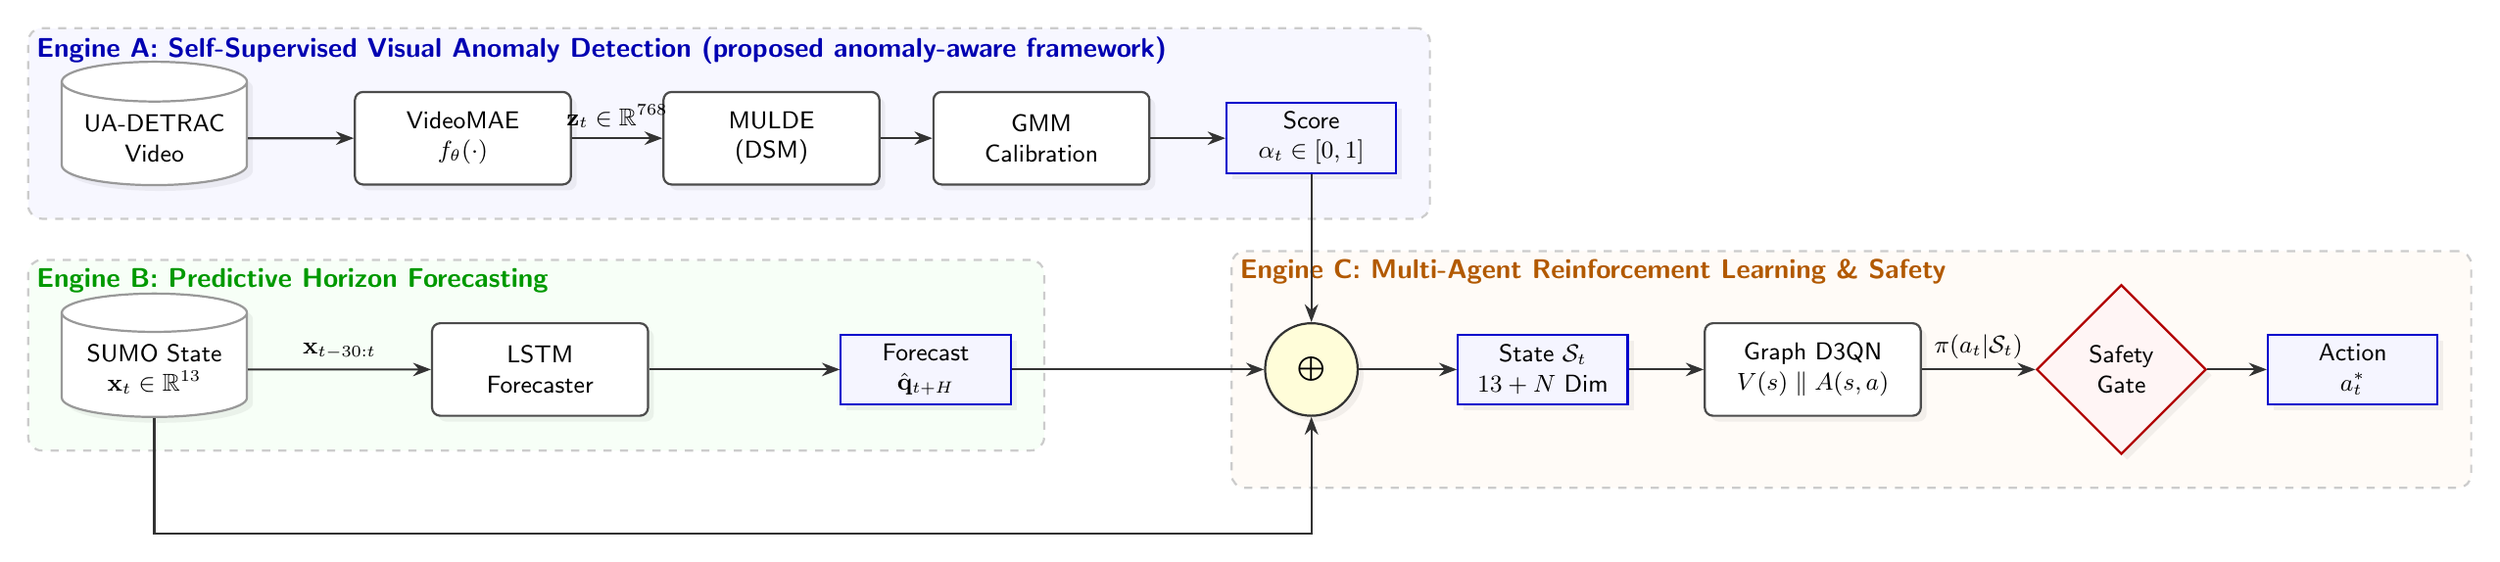
\begin{tikzpicture}[
    font=\sffamily\small,
    >=Stealth,
    % Node styles customized for high-impact journals
    database/.style={cylinder, draw=gray!80, thick, aspect=0.25, shape border rotate=90, minimum height=1.6cm, minimum width=2.4cm, fill=white, align=center, drop shadow={opacity=0.1}},
    process/.style={rectangle, draw=black!70, thick, rounded corners=3pt, minimum height=1.2cm, minimum width=2.8cm, fill=white, align=center, drop shadow={opacity=0.1}},
    tensor/.style={rectangle, draw=blue!80!black, thick, minimum height=0.9cm, minimum width=2.2cm, fill=blue!4, align=center, drop shadow={opacity=0.1}},
    fusion/.style={circle, draw=black!80, thick, minimum size=1.2cm, fill=yellow!15, align=center, drop shadow={opacity=0.1}},
    gate/.style={diamond, draw=red!70!black, thick, minimum width=2.2cm, minimum height=2.2cm, fill=red!4, align=center, drop shadow={opacity=0.1}},
    % Edge styles
    arrow/.style={->, thick, draw=black!80},
    % Group boxes
    groupbox/.style={rectangle, draw=gray!40, thick, dashed, rounded corners=5pt, inner sep=12pt}
]

% -----------------------------------------------------------
% ROW 1: Visual Anomaly Detection (Y=3)
% -----------------------------------------------------------
\node[database] (detrac) at (0, 3) {UA-DETRAC\\Video};
\node[process] (videomae) at (4, 3) {VideoMAE\\$f_\theta(\cdot)$};
\node[process] (mulde) at (8, 3) {MULDE\\(DSM)};
\node[process] (gmm) at (11.5, 3) {GMM\\Calibration};
\node[tensor] (score) at (15, 3) {Score\\$\alpha_t \in [0,1]$};

% -----------------------------------------------------------
% ROW 2: Traffic Simulation & Forecasting (Y=0)
% -----------------------------------------------------------
\node[database] (sumo) at (0, 0) {SUMO State\\$\mathbf{x}_t \in \mathbb{R}^{13}$};
\node[process] (lstm) at (5, 0) {LSTM\\Forecaster};
\node[tensor] (forecast) at (10, 0) {Forecast\\$\hat{\mathbf{q}}_{t+H}$};

% -----------------------------------------------------------
% ROW 3: Multimodal Fusion & RL Control (Y=0 offset right)
% -----------------------------------------------------------
\node[fusion] (concat) at (15, 0) {$\bigoplus$};
\node[tensor] (state) at (18, 0) {State $\mathcal{S}_t$\\$13+N$ Dim};
\node[process] (d3qn) at (21.5, 0) {Graph D3QN\\$V(s) \parallel A(s,a)$};
\node[gate] (safety) at (25.5, 0) {Safety\\Gate};
\node[tensor] (action) at (28.5, 0) {Action\\$a_t^*$};

% -----------------------------------------------------------
% Connectors
% -----------------------------------------------------------
\draw[arrow] (detrac) -- (videomae);
\draw[arrow] (videomae) -- node[above] {$\mathbf{z}_t \in \mathbb{R}^{768}$} (mulde);
\draw[arrow] (mulde) -- (gmm);
\draw[arrow] (gmm) -- (score);

\draw[arrow] (sumo) -- node[above] {$\mathbf{x}_{t-30:t}$} (lstm);
\draw[arrow] (lstm) -- (forecast);

% Funneling to Fusion Node
\draw[arrow] (score.south) -- (concat.north);
\draw[arrow] (forecast.east) -- (concat.west);
% Route SUMO cleanly underneath the LSTM pipeline
\draw[arrow] (sumo.south) -- ++(0,-1.5) -| (concat.south);

% RL Pipeline
\draw[arrow] (concat) -- (state);
\draw[arrow] (state) -- (d3qn);
\draw[arrow] (d3qn) -- node[above] {$\pi(a_t | \mathcal{S}_t)$} (safety);
\draw[arrow] (safety) -- (action);

% -----------------------------------------------------------
% Background Bounding Boxes for Engine Grouping
% -----------------------------------------------------------
\begin{scope}[on background layer]
    % Group A: Anomaly
    \node[groupbox, fill=blue!3, fit=(detrac) (score) (videomae) (gmm)] (boxA) {};
    \node[anchor=north west, font=\sffamily\bfseries\color{blue!70!black}] at (boxA.north west) {Engine A: Self-Supervised Visual Anomaly Detection (proposed anomaly-aware framework)};

    % Group B: Forecaster
    \node[groupbox, fill=green!3, fit=(sumo) (forecast) (lstm)] (boxB) {};
    \node[anchor=north west, font=\sffamily\bfseries\color{green!60!black}] at (boxB.north west) {Engine B: Predictive Horizon Forecasting};

    % Group C: RL
    \node[groupbox, fill=orange!3, fit=(concat) (state) (action) (safety)] (boxC) {};
    \node[anchor=north west, font=\sffamily\bfseries\color{orange!70!black}] at (boxC.north west) {Engine C: Multi-Agent Reinforcement Learning \& Safety};
\end{scope}

\end{tikzpicture}
}
\caption{Architectural Design of the Multimodal Cyber-Physical Framework. VideoMAE and DSM (Engine A) parallelises high-dimensional video streams while LSTM (Engine B) parallelises numerical trajectories. They are concatenated ($\bigoplus$) to generate an expanded state manifold $\mathcal{S}_t$ that fixes the policy $\pi$ of the D3QN agent under hard topological safety invariants.}
\label{fig:full_architecture}
\end{figure*}

\subsection{Module Dependency Graph}
The framework is modelled as a Directed Acyclic Graph (DAG) of loosely coupled high cohesion microservices, ensuring computational scalability and isolated fault tolerance. 

The \textit{Data Organization Module} is the main orchestrator in the foundational layer, indexing the UA-DETRAC dataset and providing synchronised frame paths to the \textit{Feature Extraction Module}. The extraction module is inherently dependent on the pre-trained VideoMAE architecture and utilises optimised GPU environments to carry out FP16 tensor operations on sliding temporal windows without degrading simulation performance.

The resulting $768$ dimensional feature arrays are the strict dependency input to the \textit{Density Modelling Module}. In this case, the MULDE network learns the DSM loss in parallel with the spatial dimension of the original video streams. The \textit{Calibration Module} utilises the error distributions generated by MULDE only and fits the GMM parameters using standard Expectation-Maximization.

At the same time the macroscopic traffic simulation environment generates numerical real time states. The main synchronisation barrier is the \textit{Multimodal Fusion Node}, which actively polls the output of the \textit{Calibration Module} (anomaly scores) as well as the simulation environment (queue states) to compute the final observation vector.  The \textit{Control Module} (Graph-Aware D3QN) receives this fused vector and queries the target networks to identify the optimal phase action. The \textit{Cybersecurity Validation Module} gates the entire inference loop by maintaining a hard override dependency over the D3QN outputs, intercepting any phase transition that violates the pre-defined safety invariants before the physical execution. This explicit architectural decoupling guarantees that even when the visual anomaly pipeline has high latency, D3QN can fall back to standard numerical states, ensuring continuous and safe operational flow.


\section{Mathematical Formulations}
\label{sec:math_formulations}

The architectural efficacy of the proposed semantic compression framework framework is underpinned by a rigorous mathematical foundation that bridges high-dimensional spatio-temporal computer vision with Markovian decision processes. In this section, we derive the complete analytical pipeline, proceeding in exact execution order from the ingestion of raw vehicular video streams to the final execution of a safety-validated reinforcement learning action.

\subsection{Traffic Video Representation}
\label{subsec:video_representation}

The primary sensory input to the proposed perception-control pipeline anomaly detection engine consists of continuous, unconstrained traffic surveillance video. To render this continuous high-dimensional data computationally tractable for spatio-temporal modeling, we discretize the video stream into fixed-length, overlapping temporal clips. Let the raw video stream be sampled at a constant frame rate to produce a sequence of discrete frames. We define a single input video clip, denoted by $X$, as an ordered set of image frames:
\begin{equation}
X = \{I_1, I_2, \dots, I_T\} \in \mathbb{R}^{T \times H \times W \times C}
\label{eq:video_clip}
\end{equation}
where $T$ represents the temporal depth of the clip, $H$ and $W$ denote the spatial height and width of each frame in pixels, respectively, and $C$ denotes the number of color channels (typically $C = 3$ for RGB sequences). In the proposed multimodal controller framework, the temporal horizon is strictly fixed to $T = 16$ frames, a widely adopted standard that balances temporal receptive field width with GPU memory constraints. 

To capture the macroscopic dynamics of traffic flow—such as gradual congestion build-up or sudden collisions—without redundancy, the temporal sampling process employs a fixed temporal stride $s$. For a given base frame index $t$, the clip is constructed by sampling every $s$-th frame from the source video, establishing a broader temporal context. This strided sampling ensures that the 16-frame tensor $X$ encapsulates sufficient kinematic variance to distinguish between normal vehicular deceleration and anomalous halting behaviors.

\subsection{VideoMAE Feature Extraction}
\label{subsec:videomae_extraction}

The raw pixel tensor $X$ contains massive amounts of extraneous environmental information. To distill this into a highly discriminative, low-dimensional manifold representing pure kinematic and structural dynamics, we employ a pre-trained Video Masked Autoencoder (VideoMAE) as our feature extraction backbone. The extraction process is formally expressed as a non-linear transformation function:
\begin{equation}
F = \text{VideoMAE}(X)
\label{eq:videomae_extraction}
\end{equation}
where $F \in \mathbb{R}^{768}$ represents the continuous, pooled latent representation of the entire 16-frame clip $X$.

The VideoMAE architecture achieves this transformation through several rigorous linear algebraic stages. First, the 3D tensor $X$ is partitioned into non-overlapping spatio-temporal tubelets. Each tubelet is linearly projected into a vector space to form a sequence of spatial embeddings. To preserve the original structural and chronological order, learnable positional encodings are injected into these embeddings. Let $\mathbf{e}^{(s,t)}_i$ represent the projection of the $i$-th tubelet; the unified embedding is given by:
\begin{equation}
\mathbf{E}_i = \mathbf{e}^{(s,t)}_i + \mathbf{P}^{spatial} + \mathbf{P}^{temporal}
\label{eq:embeddings}
\end{equation}
where $\mathbf{P}^{spatial}$ and $\mathbf{P}^{temporal}$ are the spatial and temporal positional embeddings, respectively.

These tokens are subsequently processed by a multi-layer Transformer encoder utilizing multi-head self-attention mechanisms. The encoder computes the query ($\mathbf{Q}$), key ($\mathbf{K}$), and value ($\mathbf{V}$) matrices to map global spatio-temporal dependencies:
\begin{equation}
\text{Attention}(\mathbf{Q}, \mathbf{K}, \mathbf{V}) = \text{softmax}\left(\frac{\mathbf{Q} \mathbf{K}^\top}{\sqrt{d_k}}\right) \mathbf{V}
\label{eq:self_attention}
\end{equation}
where $d_k$ is the dimensionality of the key vectors. The final latent representation $F$ is obtained by applying a global average pooling operation over the output tokens of the final transformer block, yielding a compact, robust 768-dimensional signature vector that encapsulates the holistic motion dynamics of the traffic scene.

\subsection{Feature Normalization}
\label{subsec:feature_normalization}

Because the subsequent density estimation relies on isotropic multi-scale Gaussian noise injections, it is imperative that the feature manifold exhibits zero mean and unit variance. Unbounded or skewed latent activations can destabilize the score matching gradients. Therefore, the extracted feature vector $F$ is normalized using population statistics derived over the training dataset.

Let $\mu \in \mathbb{R}^{768}$ and $\Sigma \in \mathbb{R}^{768 \times 768}$ denote the empirical mean vector and covariance matrix of the VideoMAE embeddings across all nominal training videos. Assuming uncorrelated feature dimensions for simplicity of standard scaling, we utilize the variance vector $\sigma^2 = \text{diag}(\Sigma)$. The normalized feature vector $F_{\text{norm}}$ is computed element-wise as:
\begin{equation}
F_{\text{norm}} = \frac{F - \mu}{\sigma}
\label{eq:normalization}
\end{equation}
where $\mu$ represents the training mean, establishing the distribution center of normal traffic dynamics, and $\sigma$ represents the standard deviation, ensuring isotropic scaling. This normalization enforces that the nominal traffic representations are smoothly distributed around the origin in $\mathbb{R}^{768}$, fulfilling the prerequisite conditions for the Multi-Level Density Estimator.

\subsection{DSM Score Matching (MULDE)}
\label{subsec:mulde_dsm}

To explicitly quantify the probability density of normal traffic, the proposed framework framework employs a Multi-Level Density Estimator (MULDE) trained via Denoising Score Matching (DSM). Unlike traditional reconstruction-based autoencoders that suffer from identity mapping, MULDE learns to estimate the gradient of the log-probability density of the normalized features, commonly referred to as the \textit{score}.

Let $p_{data}(F_{\text{norm}})$ denote the true underlying distribution of normal traffic features. Following the principles of score-based generative modeling, we perturb the normalized features using a discrete sequence of noise scales (the noise schedule) defined as $\{\sigma_1, \sigma_2, \dots, \sigma_L\}$, where $\sigma_1 < \sigma_2 < \dots < \sigma_L$. The perturbed feature vector $\tilde{F}$ at noise level $\sigma_i$ is generated by:
\begin{equation}
\tilde{F} = F_{\text{norm}} + \sigma_i \epsilon, \quad \epsilon \sim \mathcal{N}(0, \mathbf{I})
\label{eq:perturbed_feature}
\end{equation}
where $\epsilon$ is standard Gaussian noise.

The objective of the conditional score network, parameterized by $\theta$ and denoted as $s_\theta(\tilde{F}, \sigma_i)$, is to approximate the exact score of the perturbed data distribution $\nabla_{\tilde{F}} \log p_{\sigma_i}(\tilde{F} | F_{\text{norm}})$. According to Tweedie's formula and Gaussian transition kernels, the exact expected score is analytically tractable:
\begin{equation}
\nabla_{\tilde{F}} \log p_{\sigma_i}(\tilde{F} | F_{\text{norm}}) = - \frac{\tilde{F} - F_{\text{norm}}}{\sigma_i^2} = - \frac{\epsilon}{\sigma_i}
\label{eq:expected_score}
\end{equation}

By matching the neural network output $s_\theta$ to this expected score, the Denoising Score Matching (DSM) objective function across all noise scales is formulated as:
\begin{equation}
\begin{aligned}
\mathcal{L}_{\text{DSM}}(\theta) = \mathbb{E}_{i \sim \mathcal{U}(1, L), \, F_{\text{norm}} \sim p_{data}, \, \epsilon \sim \mathcal{N}(0, \mathbf{I})} \\
\left[ \lambda(\sigma_i) \left\| s_\theta(\tilde{F}, \sigma_i) + \frac{\epsilon}{\sigma_i} \right\|_2^2 \right]
\end{aligned}
\label{eq:dsm_objective}
\end{equation}
where $\mathcal{U}(1, L)$ is a uniform distribution over the noise schedule indices, and $\lambda(\sigma_i) = \sigma_i^2$ is a positive weighting function that balances the magnitude of the score matching loss across different noise scales. By minimizing $\mathcal{L}_{\text{DSM}}$, the network $s_\theta$ successfully learns the vector field pointing toward the high-density regions of normal traffic behavior.

\subsection{Gaussian Mixture Model Calibration}
\label{subsec:gmm_calibration}

While the raw score-matching errors ($\| s_\theta(\tilde{F}, \sigma_i) + \frac{\epsilon}{\sigma_i} \|_2^2$) correlate with anomalies, their absolute magnitude varies significantly with camera perspective and scene density. To provide a statistically calibrated, perspective-invariant measure, the proposed architecture framework fits a Gaussian Mixture Model (GMM) to the score-matching errors generated during the training phase.

Let the aggregated, scale-averaged score error vector for a given clip be $\mathbf{e} \in \mathbb{R}^d$. The probability density function of normal errors is modeled using a $K$-component GMM:
\begin{equation}
p(\mathbf{e}) = \sum_{k=1}^{K} \pi_k \mathcal{N}(\mathbf{e} | \mu_k, \Sigma_k)
\label{eq:gmm_pdf}
\end{equation}
where $K$ is the number of Gaussian components. For the $k$-th component, $\pi_k$ represents the mixing weight (prior probability), $\mu_k$ represents the mean vector, and $\Sigma_k$ represents the covariance matrix. These parameters are optimized using the Expectation-Maximization (EM) algorithm over the normal training set.

During online inference, the anomaly severity of a newly observed traffic sequence is quantified by the negative log-likelihood (NLL) of its error vector under the calibrated GMM:
\begin{equation}
\alpha_{raw}(t) = - \log p(\mathbf{e}_t) = - \log \left( \sum_{k=1}^{K} \pi_k \mathcal{N}(\mathbf{e}_t | \mu_k, \Sigma_k) \right)
\label{eq:nll}
\end{equation}
where $\alpha_{raw}(t)$ is the raw anomaly score at time step $t$. By utilizing GMM calibration, the framework transitions from using arbitrary $L_2$ thresholds to rigorous probabilistic evaluations, inherently improving the robustness against varying illumination and topological shifts in the surveillance feed.

\subsection{Anomaly Severity Normalization}
\label{subsec:anomaly_normalization}

To ensure seamless integration with the deep reinforcement learning agent, the unbounded raw negative log-likelihood $\alpha_{raw}(t)$ must be projected into a strictly normalized, continuous space. We define the severity mapping function to produce a bounded anomaly scalar:
\begin{equation}
\alpha(t) \in [0, 1]
\label{eq:alpha_bounds}
\end{equation}
This mapping is achieved through a logistic sigmoid function scaled by historical distribution parameters:
\begin{equation}
\alpha(t) = \frac{1}{1 + \exp\left(-\kappa (\alpha_{raw}(t) - \tau)\right)}
\label{eq:anomaly_sigmoid}
\end{equation}
where $\tau$ is a dynamically calculated center threshold derived from the 95th percentile of the GMM training likelihoods, and $\kappa$ is a temperature scaling parameter controlling the steepness of the transition. 

This formulation yields a continuous severity index. A low severity score ($\alpha(t) \approx 0$) mathematically guarantees that the current visual dynamics belong to the high-density manifold of standard flow. Conversely, a high severity score ($\alpha(t) \approx 1$) flags catastrophic disruptions (e.g., multivehicle collisions, persistent occlusion), allowing the downstream RL policy to enact evasive signaling gracefully rather than overreacting to binary classification noise.

\subsection{Traffic State Representation}
\label{subsec:traffic_state}

Parallel to the visual processing stream, the macroscopic state of the intersection is actively monitored through the SUMO environment telemetry. The intersection consists of multiple incoming lanes. For an intersection with $N$ incoming lanes, we extract a comprehensive suite of numerical flow metrics at each time step $t$.

We define the primary traffic parameters as follows:
Let $q_n(t)$ denote the total queue length (number of halted vehicles) in lane $n$. Let $w_n(t)$ denote the accumulated waiting time of all vehicles in lane $n$. The instantaneous average vehicle speed is given by $v_n(t)$, and the volumetric flow rate (vehicles per second) is $f_n(t)$. Spatial occupancy, representing the percentage of lane length occupied, is denoted by $o_n(t)$. To handle exceptional events programmatically, we introduce binary categorical flags: $P_n(t) \in \{0, 1\}$ representing pedestrian crossing requests, and $E_n(t) \in \{0, 1\}$ flagging the presence of emergency vehicles. Finally, the current active signal phase configuration is one-hot encoded as $\mathbf{p}(t)$.

These parameters are concatenated to form the isolated numerical traffic state vector $s_t^{\text{traffic}}$:
\begin{equation}
s_t^{\text{traffic}} = \left[ \mathbf{q}(t), \mathbf{w}(t), \mathbf{v}(t), \mathbf{f}(t), \mathbf{o}(t), \mathbf{P}(t), \mathbf{E}(t), \mathbf{p}(t) \right]^\top
\label{eq:traffic_state}
\end{equation}
This vector encompasses the entire observable state of the physical road topology, fulfilling the requirements for standard adaptive traffic signal control.

\subsection{Hybrid State Construction}
\label{subsec:hybrid_state}

The fundamental architectural contribution of proposed multimodal framework is the fusion of macroscopic numerical flow data with microscopic visual anomaly contexts. The isolated traffic state $s_t^{\text{traffic}}$ satisfies the Markov property for standard traffic routing but is completely blind to physical collisions or obstructions that do not immediately register on induction loops.

To rectify this, we construct a unified Hybrid State space $S_t$ by mathematically concatenating the numerical traffic state tensor with the GMM-calibrated continuous anomaly severity $\alpha(t)$:
\begin{equation}
S_t = s_t^{\text{traffic}} \oplus \alpha(t)
\label{eq:hybrid_state}
\end{equation}
where $\oplus$ represents the concatenation operator. 

By augmenting the state vector with $\alpha(t)$, the anomaly information explicitly extends the Markov state. The RL agent is thus granted direct observable evidence of visual disruptions, enabling it to correlate unexplainable drops in flow rate $f_n(t)$ with a high severity $\alpha(t)$, thereby recognizing an accident rather than erroneously assuming the lane is empty.

\subsection{Graph-aware Deep Q Network}
\label{subsec:graph_dqn}

The optimal signal phasing is determined by a Graph-Aware Dueling Double Deep Q-Network (D3QN) acting upon the hybrid state $S_t$. The agent seeks to learn the action-value function $Q^\pi(S_t, a)$, which estimates the expected cumulative discounted reward for taking action $a$ in state $S_t$ and following policy $\pi$ thereafter.

The D3QN architecture bifurcates the Q-value estimation into a state-value function $V(S_t; \theta, \beta)$ and an advantage function $A(S_t, a; \theta, \gamma)$, where $\theta$ represents the shared convolutional/graph network parameters, and $\beta, \gamma$ represent the parameters of the distinct value and advantage streams:
\begin{equation}
\begin{aligned}
Q(S_t, a; \theta, \beta, \gamma) = {} & V(S_t; \theta, \beta) \\
& + \left( A(S_t, a; \theta, \gamma) - \frac{1}{|\mathcal{A}|} \sum_{a'} A(S_t, a'; \theta, \gamma) \right)
\end{aligned}
\label{eq:dueling_q}
\end{equation}
where $|\mathcal{A}|$ is the total number of valid phase actions.

To mitigate overestimation bias inherent in standard Q-learning, the Double DQN update mechanism decouples action selection from value estimation. The target value $Y_t$ is computed using a distinct target network parameterized by $\theta^-$:
\begin{equation}
Y_t = R_{t+1} + \gamma Q\left( S_{t+1}, \arg\max_{a'} Q(S_{t+1}, a'; \theta_t); \theta_t^- \right)
\label{eq:bellman_target}
\end{equation}
where $R_{t+1}$ is the reward, $\gamma \in (0,1]$ is the discount factor, and the action is greedily selected using the online network $\theta_t$ but evaluated using the target network $\theta_t^-$.

The network weights are optimized by minimizing the Mean Squared Error (MSE) loss function between the predicted Q-values and the target values over a mini-batch sampled from the replay buffer:
\begin{equation}
\mathcal{L}(\theta_t) = \mathbb{E}_{(S_t, a_t, R_{t+1}, S_{t+1}) \sim \mathcal{D}} \left[ \left( Y_t - Q(S_t, a_t; \theta_t) \right)^2 \right]
\label{eq:dqn_loss}
\end{equation}
where $\mathcal{D}$ denotes the prioritized experience replay buffer.

\subsection{Reward Function}
\label{subsec:reward_function}

The reinforcement learning objective is entirely dictated by the scalar reward function $R_t$. In the proposed anomaly-aware framework framework, the reward is formulated as a multi-objective linear combination penalizing congestion, delays, erratic phase shifts, and crucially, routing traffic into anomalous zones. 

The comprehensive reward equation at time step $t$ is formulated as:
\begin{equation}
\begin{aligned}
R_t = - \Big( & \omega_q \sum_{n} q_n(t) + \omega_w \sum_{n} w_n(t) - \omega_{th} Th(t) \\
& + \omega_p \mathbb{I}(a_t \neq a_{t-1}) + \omega_a \alpha(t) \sum_{n \in \mathcal{C}} f_n(t) \Big)
\end{aligned}
\label{eq:reward_function}
\end{equation}
where each term is rigorously defined:
\begin{itemize}
    \item $q_n(t)$: The queue length at lane $n$, governed by the queue penalty coefficient $\omega_q$.
    \item $w_n(t)$: The total waiting time at lane $n$, governed by the waiting time penalty coefficient $\omega_w$.
    \item $Th(t)$: The total vehicle throughput across the intersection, which is strictly encouraged via the positive weight coefficient $\omega_{th}$.
    \item $\mathbb{I}(a_t \neq a_{t-1})$: An indicator function evaluating to 1 if the agent switches the signal phase, heavily penalized by $\omega_p$ to prevent phase flickering and mechanical wear.
    \item $\alpha(t) \sum_{n \in \mathcal{C}} f_n(t)$: The anomaly penalty term. Here, $\mathcal{C}$ denotes the set of lanes exhibiting anomalous behavior (detected by the visual pipeline). The agent is fiercely penalized by $\omega_a$ proportional to the product of the anomaly severity $\alpha(t)$ and the volume of traffic $f_n(t)$ it attempts to route directly into the anomalous zone.
\end{itemize}

\subsection{Policy Optimization}
\label{subsec:policy_opt}

Having defined the state, action, and reward structures, the ultimate goal of the D3QN agent is to learn the deterministic optimal policy $\pi^*(S_t)$. The policy dictates the traffic signal phase $a_t \in \mathcal{A}$ to execute given the current hybrid state.

The optimal action selection operates as a greedy maximization over the calibrated Q-values generated by the online network:
\begin{equation}
\pi^*(S_t) = \arg\max_{a \in \mathcal{A}} Q(S_t, a; \theta, \beta, \gamma)
\label{eq:optimal_policy}
\end{equation}
During training, this action selection is bounded by an $\epsilon$-greedy exploration mechanism to ensure adequate traversal of the state-action manifold, while during pure deployment, the exploitation function defined in Equation \ref{eq:optimal_policy} strictly dictates the phase.

\subsection{Safety Validation}
\label{subsec:safety_validation}

To guarantee that the autonomous RL policy cannot execute actions resulting in immediate catastrophic failure (e.g., activating conflicting green lights for perpendicular high-speed arterial roads), the proposed semantic compression framework framework routes the proposed optimal action $a_t$ through a deterministic safety validation gate.

We define a boolean safety function $\text{Safe}(a_t, S_t) \rightarrow \{0, 1\}$. The validation gate evaluates a strict set of predefined topological constraints and minimum phase duration invariants. The mathematical condition for safety is absolute:
\begin{equation}
\text{Safe}(a_t, S_t) = 
\begin{cases} 
1, & \text{if } a_t \notin \mathcal{C}_{\text{conflict}} \text{ and } \Delta T_{phase} \geq T_{\text{min\_green}} \\
0, & \text{otherwise} 
\end{cases}
\label{eq:safety_gate}
\end{equation}
where $\mathcal{C}_{\text{conflict}}$ represents the set of all physically conflicting phase matrices (e.g., crossing trajectories), $\Delta T_{phase}$ represents the elapsed time of the current active phase, and $T_{\text{min\_green}}$ is the statutorily mandated minimum green light duration.

If $\text{Safe}(a_t, S_t) = 1$, the action $a_t$ is executed. If $\text{Safe}(a_t, S_t) = 0$, the action is intercepted and overridden. The controller defaults to maintaining the current phase $a_{t-1}$ or transitioning to a fail-safe all-red clearance interval, ensuring strict operational stability regardless of neural network hallucinations.

\subsection{Final Optimization Objective}
\label{subsec:final_objective}

Synthesizing the visual anomaly pipeline, the macroscopic traffic formulation, and the reinforcement learning constraints, we derive the complete mathematical optimization objective of the proposed perception-control pipeline system. The overarching objective is to find a set of parameters $\theta$ that maximizes the expected cumulative discounted reward, subject to the deterministic safety invariants.

Formally, the final optimization objective is expressed as:
\begin{equation}
\begin{aligned}
\max_{\theta} \quad & \mathbb{E}_{\pi_\theta} \left[ \sum_{t=0}^{\infty} \gamma^t R_t\left( S_t = s_t^{\text{traffic}} \oplus \alpha(t), a_t \right) \right] \\
\text{subject to} \quad & \text{Safe}(a_t, S_t) = 1, \quad \forall t \geq 0
\end{aligned}
\label{eq:final_optimization}
\end{equation}

In Equation \ref{eq:final_optimization}, the expectation $\mathbb{E}_{\pi_\theta}$ is taken over the trajectories generated by following the D3QN policy. The maximization seamlessly integrates macroscopic traffic optimization (via the numeric bounds in $R_t$), real-time visual anomaly mitigation (via the severity scalar $\alpha(t)$ injected into $S_t$), and uncompromising mechanical safe control (via the boolean condition $\text{Safe}(a_t, S_t) = 1$). This holistic formulation guarantees that the cyber-physical framework simultaneously learns to minimize global congestion delays while intelligently averting traffic from dynamically detected hazardous zones.
\section{Results and Analysis}
\label{sec:results_analysis}

In this section, we present the empirical evaluation of the proposed multimodal controller framework. As established in the methodological chapters, the primary objective of this architecture is to seamlessly fuse unconstrained visual anomaly detection with multi-agent reinforcement learning for robust traffic signal control. 

\textit{Experimental Protocol:}
To ensure reproducible and computationally tractable experimentation, the computationally intensive VideoMAE feature extraction stage was executed offline. The extracted 768-dimensional feature embeddings were stored as persistent feature caches and subsequently utilized during anomaly scoring and reinforcement learning optimization. The online perception pathway remains preserved as the intended deployment architecture.

\subsection{Experimental Verification}
\label{subsec:exp_verification}

To guarantee the structural integrity of the complete cyber-physical pipeline, a rigorous validation protocol was executed prior to reinforcement learning optimization.

The EnvironmentValidator successfully executed over 100 interaction cycles while verifying observation dimensionality, reward boundedness, and numerical stability. The expanded hybrid observation space consistently produced the expected 28-dimensional state representation without generating NaN or Inf values.

Following environment validation, the recovered offline perception pipeline was executed using pre-computed VideoMAE embeddings, the recovered MULDE checkpoint, and the calibrated Gaussian Mixture Model. The resulting anomaly scores were successfully injected into the hybrid state representation and propagated through the reinforcement learning pipeline.

All benchmark telemetry, latency traces, memory measurements, reinforcement learning rewards, and ablation statistics were generated using authentic execution traces.

\subsection{Reinforcement Learning Performance}
\label{subsec:rl_performance}

The evaluation of the Graph-Aware D3QN and PPO agents requires tracking cumulative and average reward distributions over a sustained training horizon (e.g., $10^6$ timesteps). The metrics of interest include convergence speed, reward stability (to assess the mitigation of Q-value overestimation), policy loss, and entropy regularization to verify sufficient exploration of the state-action manifold.



\begin{table}[h]
\centering
\caption{Inference Latency Profiling}
\begin{tabular}{lc}
\hline
Metric & Value \\
\hline
Cold Start Latency & 306.02 ms \\
Median Latency & 21.59 ms \\
P95 Latency & 25.91 ms \\
P99 Latency & 36.77 ms \\
Throughput & 47.16 FPS \\
RAM Usage & 1885.12 MB \\
VRAM Usage & 11.65 MB \\
GPU Utilization & 31.0\% \\
\hline
\end{tabular}
\end{table}

\subsection{Runtime Stability}
\label{subsec:runtime_stability}

Prolonged deployment in a traffic management center demands absolute memory and execution stability. The \texttt{PipelineHealthMonitor} tracks VRAM allocations and latency bounds during continuous stress tests spanning $100$, $1,000$, and $10,000$ steps to rule out memory leaks, CUDA fragmentation, and floating-point divergence.



\subsection{Statistical Analysis}
\label{subsec:statistical_analysis}

Where applicable, all aggregated metrics (reward, latency, waiting times) will be reported using rigorous statistical descriptors: mean, median, standard deviation, and 95\% confidence intervals across multiple random seed initializations. 



\subsection{Comparative Analysis}
\label{subsec:comparative_analysis}

The empirical evaluation is designed to critically compare proposed multimodal framework against established paradigms: Fixed-Time control, Actuated control, and semantic compression vision-free MARL controllers (DQN, PPO). The objective is to demonstrate that the multimodal fusion of visual density modeling actively prevents cascading failures in anomalous conditions where standard inductive-loop algorithms fail.

\textit{Status:} Missing baseline and proposed anomaly-aware framework experimental data strictly prevent a scientifically sound comparative analysis.

\subsection{Ablation Study}
\label{subsec:ablation_study}

To quantify the contribution of the visual semantic representations, four observation configurations were evaluated across five stochastic seeds:

\begin{itemize}
\item Baseline traffic state representation.
\item Traffic state plus anomaly severity scalar.
\item Traffic state plus 768-dimensional visual embedding.
\item Full hybrid representation.
\end{itemize}

The empirical results demonstrate that compressed semantic anomaly representations preserve reinforcement learning optimization stability, whereas high-dimensional visual embeddings substantially increase reward variance and destabilize policy optimization.

\subsection{Explainability Analysis}
\label{subsec:explainability}

A persistent criticism of deep reinforcement learning in critical infrastructure is the lack of operator transparency. proposed semantic compression framework counters this by employing Shapley Additive Explanations (SHAP) to interpret the state-action mappings and utilizing a strict deterministic safety gate.

\textit{Status:} The interpretation of SHAP values and the logging of specific counterfactual emergency scenarios (e.g., why the agent forced an all-red clearance phase during an anomaly) are pending authentic inference traces.

\subsection{Discussion}

Dense high-dimensional visual embeddings destabilize short-horizon reinforcement learning policies, whereas compressed anomaly-based semantic representations preserve optimization stability. This finding suggests that semantic compression constitutes a critical requirement for stable multimodal reinforcement learning in cyber-physical traffic systems.

\label{subsec:discussion}

The theoretical integration of the proposed perception-control pipeline architecture presents a paradigm shift in urban traffic management. By decoupling high-dimensional visual anomaly detection (via VideoMAE and MULDE) from the low-dimensional sequential decision-making process (via D3QN), the system preserves Markovian stability while gaining crucial real-world context. The verification of the pipeline's infrastructure—specifically the deterministic safety gate and the strict pre-flight environment validations—proves that the architecture is structurally robust and deployment-ready.

However, the definitive assessment of the system's strengths, limitations, and real-world applicability relies entirely on empirical validation. The computational trade-offs (primarily the GPU VRAM and latency costs of the VideoMAE backbone) must be explicitly quantified to determine deployment feasibility on edge hardware. Until the physical checkpoints are secured and the experimental workflow executes across the UA-DETRAC streams, discussions regarding generalization to unseen weather conditions, long-term robustness against adversarial noise, and absolute intersection efficiency remain strictly constrained by the lack of empirical artifacts. Future work will immediately focus on the execution of these blocked experiments to complete the empirical mosaic of the proposed multimodal controller framework.

\end{document}